\begin{center}
\footnotesize\noindent\fbox{
	\parbox{\textwidth}{
	Utilizzare le functions degli esercizi precedenti per disegnare l'approssimazione della funzione \(\sin(x)\) nell'intervallo \([0, 2\pi]\), utilizzando le ascisse di interpolazione \(x_i=i\pi\), \(i= 0,1,2\).
	}
}\end{center}

\noindent Nell'immagine seguente si pu\'o vedere in blu il grafico della funzione \(\sin(x)\), mentre in rosso il grafico del polinomio interpolante costruito date le ascisse \(0, \pi, 2\pi \).
\begin{center}
	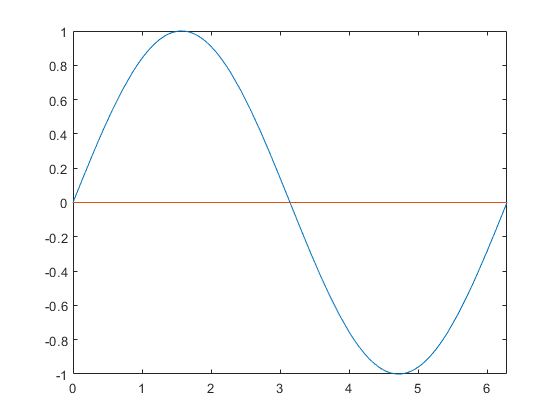
\includegraphics[scale=0.7]{cap4/4-4.png}
\end{center}
\noindent Come si nota facilmente, il polinomio interpolante in reallt\'a \'e la retta delle ascisse \(y=0\). Questo perch\'e la funzione \(y = \sin(x)\) nei tre punti di ascissa dati \(0, \pi, 2\pi \) vale zero, pertanto i coefficienti del polinomio interpolante risultano tutti nulli. \\ \\
\noindent Di seguito il codice Matlab usato per realizzare il grafico precedente. Si noti che \'e stato usato il polinomio interpolante di Newton per ottenere l'approssimazione della funzione, ma

HERMITE???
